% ------------------------------------------------------------------------------
% TYPO3 CMS 8.4 - What's New - Chapter "Deprecated Functions" (French Version)
%
% @author	Michael Schams <schams.net>
% @license	Creative Commons BY-NC-SA 3.0
% @link		http://typo3.org/download/release-notes/whats-new/
% @language	French
% ------------------------------------------------------------------------------
% LTXE-CHAPTER-UID:		3f842373-9262b8d3-f9c8de76-cf29ce17
% LTXE-CHAPTER-NAME:	Fonctions dépréciées
% ------------------------------------------------------------------------------

\section{Fonctions dépréciées et retirées}
\begin{frame}[fragile]
	\frametitle{Fonctions dépréciées et retirées}

	\begin{center}\huge{Chapitre 5~:}\end{center}
	\begin{center}\huge{\color{typo3darkgrey}\textbf{Fonctions dépréciées et retirées}}\end{center}

\end{frame}

% ------------------------------------------------------------------------------
% LTXE-SLIDE-START
% LTXE-SLIDE-UID:		fa8cb76f-7f1deda9-37723b33-6bd56074
% LTXE-SLIDE-ORIGIN:	cf7400eb-0f683329-f6c51cbf-dfd192d9 English
% LTXE-SLIDE-TITLE:		#77630: Remove wizard icons
% ------------------------------------------------------------------------------
\begin{frame}[fragile]
	\frametitle{Fonctions dépréciées et retirées}
	\framesubtitle{Icônes d'assitant retirés}

	\begin{itemize}

		\item Les icônes suivants sont retirés de FormFieldWizard~:

			\begin{itemize}
				\item \texttt{wizard\_add.gif}
				\item \texttt{wizard\_edit.gif}
				\item \texttt{wizard\_link.gif}
				\item \texttt{wizard\_list.gif}
				\item \texttt{wizard\_rte.gif}
				\item \texttt{wizard\_table.gif}
			\end{itemize}

	\end{itemize}

	\begin{figure}
		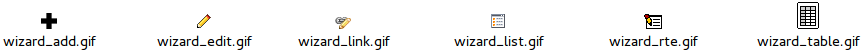
\includegraphics[width=0.95\linewidth]{DeprecatedRemovedFunctions/77630.png}
	\end{figure}

\end{frame}

% ------------------------------------------------------------------------------
% LTXE-SLIDE-START
% LTXE-SLIDE-UID:		b7ac976e-78c33b1d-40780bdb-ab757001
% LTXE-SLIDE-ORIGIN:	d5ced5e7-04dffe16-b8ec9f2c-712020cd English
% LTXE-SLIDE-TITLE:		#77693: Remove/Move Icons from EXT:t3skin
% ------------------------------------------------------------------------------

\begin{frame}[fragile]
	\frametitle{Fonctions dépréciées et retirées}
	\framesubtitle{Icônes de \texttt{EXT:t3skin}}

	\begin{itemize}

		\item Des icônes de \texttt{EXT:t3skin} sont retirés ou déplacés
		\item \textbf{Retirés~:}

			\begin{itemize}
				\item \smaller\texttt{typo3/sysext/t3skin/icons/gfx/error.png}
				\item \texttt{typo3/sysext/t3skin/icons/gfx/i/\_icon\_ftp.gif}
				\item \texttt{typo3/sysext/t3skin/icons/gfx/information.png}
				\item \texttt{typo3/sysext/t3skin/icons/gfx/notice.png}
				\item \texttt{typo3/sysext/t3skin/icons/gfx/warning.png}
			\end{itemize}

		\item \textbf{Déplacés~:}

			\begin{itemize}
				\item \smaller\texttt{typo3/sysext/t3skin/icons/gfx/icon\_fatalerror.gif}
				\item \texttt{typo3/sysext/t3skin/images/icons/status/status-edit-read-only.png}
				\item \texttt{typo3/sysext/t3skin/images/icons/status/warning-in-use.png}
				\item \texttt{typo3/sysext/t3skin/images/icons/status/warning-lock.png}
				\item \texttt{typo3/sysext/t3skin/images/icons/status/status-reference-hard.png}
				\item \texttt{typo3/sysext/t3skin/images/icons/status/status-reference-soft.png}
			\end{itemize}

	\end{itemize}

\end{frame}

% ------------------------------------------------------------------------------
% LTXE-SLIDE-START
% LTXE-SLIDE-UID:		1f175e52-d5d67741-566f6d94-af2ab6fc
% LTXE-SLIDE-ORIGIN:	7848f0b0-d687b337-f7638646-680dc819 English
% LTXE-SLIDE-TITLE:		Obsolete page tree and click menu settings removed
% ------------------------------------------------------------------------------

\begin{frame}[fragile]
	\frametitle{Fonctions dépréciées et retirées}
	\framesubtitle{Options de l'arborescence et du menu au clic}

	\begin{itemize}

		\item Les options obsolètes de l'arborescence des pages et du menu au clic sont retirées
		\item \textbf{Propriétés}~:

		\begin{itemize}
			\item \texttt{FileSystemNavigationFrameController->doHighlight}
			\item \texttt{ClickMenu->leftIcons}
		\end{itemize}

		\item \textbf{Options TypoScript}~:

		\begin{itemize}
			\item \texttt{options.pageTree.disableTitleHighlight}
			\item \texttt{options.contextMenu.options.leftIcons}
		\end{itemize}

	\end{itemize}

\end{frame}

% ------------------------------------------------------------------------------
% LTXE-SLIDE-START
% LTXE-SLIDE-UID:		cdebd43e-a5daad8b-a9fcffd8-b1cc30e5
% LTXE-SLIDE-ORIGIN:	aad23a73-7b046eaf-fb4bb862-2f88ef71 English
% LTXE-SLIDE-TITLE:		ExtensionManagementUtility::extRelPath()
% LTXE-SLIDE-REFERENCE:	#78193: ExtensionManagementUtility::extRelPath() deprecated
% ------------------------------------------------------------------------------

\begin{frame}[fragile]
	\frametitle{Fonctions dépréciées et retirées}
	\framesubtitle{ExtensionManagementUtility::extRelPath()}

	\begin{itemize}

		\item La méthode \texttt{ExtensionManagementUtility::extRelPath()} est marquée dépréciée
		\item Elle était utilisée pour calculer les chemins relatifs au script actuel
		\item Méthodes alternatives disponibles~:

			\begin{itemize}
				\item \texttt{ExtensionManagementUtility::extPath()}\newline
					(pour obtenir le chemin complet d'une extension)
				\item \texttt{ExtensionManagementUtility::siteRelPath()}\newline
					(pour obtenir le chemin d'une extension par rapport à \texttt{PATH\_site}
				\item \texttt{GeneralUtility::getFileAbsFileName()}\newline
					(pour obtenir le chemin réel à partir d'un chemin préfixé par EXT:myextension)
				\item \texttt{PathUtility::getAbsoluteWebPath()}\newline
					(pour obtenir l'URL absolue d'un fichier pour le Web)
			\end{itemize}

	\end{itemize}

\end{frame}

% ------------------------------------------------------------------------------
% LTXE-SLIDE-START
% LTXE-SLIDE-UID:		321f860d-926f57ef-ec776530-522aea03
% LTXE-SLIDE-ORIGIN:	43a5eaf5-8945a8d5-ac27d4ea-24ffc8e3 English
% LTXE-SLIDE-TITLE:		Miscellaneous (1) (#75363)
% LTXE-SLIDE-REFERENCE:	#75363: Deprecate FormResultCompiler->JStop()
% LTXE-SLIDE-REFERENCE:	#75637: Deprecate optional parameters of RecyclerUtility::getRecordPath()
% ------------------------------------------------------------------------------

\begin{frame}[fragile]
	\frametitle{Fonctions dépréciées et retirées}
	\framesubtitle{Divers (1)}

	\begin{itemize}
		\item La méthode \texttt{FormResultCompiler->JStop()} est renommée \texttt{addCssFiles()}.
			L'ancienne méthode reste disponible en tant qu'alias déprécié, qui sera retirée en v9.

		\item La méthode \texttt{ClickMenu::DB\_editPageProperties()} est marquée dépréciée

		\item Les arguments suivants de la méthode \texttt{RecyclerUtility::getRecordPath()}
			sont marqués dépréciés~:

			\begin{itemize}
				\item \texttt{\$clause}
				\item \texttt{\$titleLimit}
				\item \texttt{\$fullTitleLimit}
			\end{itemize}

	\end{itemize}

\end{frame}

% ------------------------------------------------------------------------------
% LTXE-SLIDE-START
% LTXE-SLIDE-UID:		fbb4fdfc-92e19cfc-79205738-d461d0a2
% LTXE-SLIDE-ORIGIN:	0745e3f3-83db03d7-ac24e92a-300391ba English
% LTXE-SLIDE-TITLE:		Miscellaneous (2) (#77783 and #77826)
% LTXE-SLIDE-REFERENCE:	#77783: Unused ExtJS JavaScript libraries removed
% LTXE-SLIDE-REFERENCE:	#77826: RTEHtmlArea Spellchecker eID removed
% ------------------------------------------------------------------------------

\begin{frame}[fragile]
	\frametitle{Fonctions dépréciées et retirées}
	\framesubtitle{Divers (2)}

	\begin{itemize}

		\item Les bibliothèques ExtJS non-utilisées suivantes sont retirées~:

			\begin{itemize}
				\item \texttt{app.SearchField}
				\item \texttt{grid.RowExpander}
				\item \texttt{ux.FitToParent}
			\end{itemize}

		\item L'eID de RTEHtmlArea (\texttt{rtehtmlarea\_spellchecker}) pour
			utiliser la correction orthographique dynamique est retiré et le point d'entrée des requêtes HTTP
			\texttt{SpellCheckingController->main} marqué comme déprécié

		\item Le format \texttt{DateTime::ISO8601} est incompatible avec ISO-8601,
			mais est gardé pour la compatibilité.
			Les constantes \texttt{DateTime::ATOM} ou \texttt{DATE\_ATOM} sont utilisées à la place.

	\end{itemize}

\end{frame}

% ------------------------------------------------------------------------------
% LTXE-SLIDE-START
% LTXE-SLIDE-UID:		dfa08209-c53cc091-93991bba-c5a5b705
% LTXE-SLIDE-ORIGIN:	0745e3f3-83db03d7-ac24e92a-300391ba English
% LTXE-SLIDE-TITLE:		Miscellaneous (3) (#77839, #78096 and #78222)
% LTXE-SLIDE-REFERENCE:	#77839: TYPO3/CMS/Core/QueryGenerator
% LTXE-SLIDE-REFERENCE:	#78096: Deprecate PageLayoutView::getResult with mysqli_result objects
% LTXE-SLIDE-REFERENCE:	#78222: Late generation of autoload information is deprecated
% ------------------------------------------------------------------------------

\begin{frame}[fragile]
	\frametitle{Fonctions dépréciées et retirées}
	\framesubtitle{Divers (3)}

	\begin{itemize}

		\item Le module AMD \texttt{TYPO3/CMS/Core/QueryGenerator} est déplacé dans EXT:lowlevel\newline
			\small
				(et renommé en \texttt{TYPO3/CMS/Lowlevel/QueryGenerator})
			\normalsize

		\item La méthode \texttt{PageLayoutView::getResult()} est marquée dépréciée lors de
			l'usage d'un objet \texttt{mysqli\_result} comme premier paramètre

		\item Lors de l'usage de TYPO3 en mode non-composer, la génération des informations
			de chargement des classes était effectuée durant l'initialisation. Ce comportement
			est déprécié.
	\end{itemize}

\end{frame}

% ------------------------------------------------------------------------------
